% command to run this on the terminal is lualatex -shell-escape Pictogram_Sleep_Regulation.tex
% requires pgfplots

\pdfpxdimen=1in
\divide\pdfpxdimen by 600

\documentclass[10pt]{standalone}
\usepackage{tikz}
%has to be compiled with ``lualatex -shell-escape Pictogram_TC.tex''
\usetikzlibrary{external, positioning, backgrounds, arrows.meta,decorations.pathmorphing}

% set up externalization
%\tikzexternalize[prefix=tikz/]
% WARNING the name of the Image CANNOT be the same as the tex file
\tikzsetnextfilename{Pictogram_TC}
\tikzset{external/system call={lualatex \tikzexternalcheckshellescape -halt-on-error
-interaction=batchmode -jobname "\image" "\texsource";
convert -density 600 -compress LZW "\image".pdf -flatten -alpha off -colorspace RGB -depth 8 "\image".tif;
convert -density 600 "\image".tif  "\image".jpg;}}
\tikzexternalize

\begin{document}
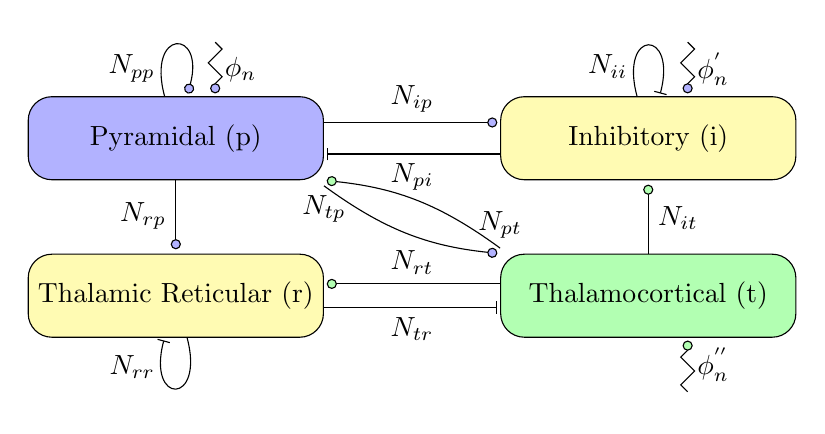
\begin{tikzpicture}[
  s/.style  = {shorten >=1pt},
  every loop/.style={shorten >=1pt},
  pop/.style	 = {rectangle, draw, text width=10em, text centered, minimum height=3em, rounded corners=3mm},
  noise_C/.style = {decorate, decoration={zigzag}, s,-{Circle[fill=blue!30]}},
  noise_T/.style = {decorate, decoration={zigzag}, s,-{Circle[fill=green!30]}},
  Ex/.style = {rounded corners, s, -{Circle[fill=blue!30]}},
  Tc/.style = {rounded corners, s, -{Circle[fill=green!30]}},
  In/.style = {rounded corners, s, -|},
  ]

  % Cortex populations
  \node (ex)   at (0,0)	 [pop, fill=blue!30]	{Pyramidal (p)};
  \node (in)   at (6,0)	 [pop, fill=yellow!30]	{Inhibitory (i)};
  % Thalamus Populations
  \node (tc)   at (6,-2) [pop, fill=green!30]	{Thalamocortical (t)};
  \node (re)   at (0,-2) [pop, fill=yellow!30]	{Thalamic Reticular (r)};

  % Connections within cortex
  \draw
  (		   ex)	    edge [Ex, loop above] node[below left, xshift = -0.4em]	{$N_{pp}$}	(		ex)
  ([yshift= 0.2cm] ex.east) edge [Ex]		  node[above] 				{$N_{ip}$}	([yshift= 0.2cm]in.west)
  ([yshift=-0.2cm] in.west) edge [In] 	    	  node[below] 				{$N_{pi}$}	([yshift=-0.2cm]ex.east)
  (		   in)	    edge [In, loop above] node[below left, xshift = -0.4em]	{$N_{ii}$}	(		in)
  (0.5,1.22)  		    edge [noise_C] 	  node[right] 				{$\phi_n$}	([xshift= 0.5cm]ex.north)
  (6.5,1.22)  		    edge [noise_C] 	  node[right] 				{$\phi^{'}_n$}	([xshift= 0.5cm]in.north);

  % Connections within thalamus
  \draw
  (6.5,-3.22)               edge [noise_T]	  node[right] 				{$\phi^{''}_{n}$}([xshift=0.5cm]  tc.south)
  ([yshift= 0.15cm]tc.west) edge [Tc]	 	  node[above]				{$N_{rt}$}	([yshift= 0.15cm] re.east)
  ([yshift=-0.15cm]re.east) edge [In]	 	  node[below]				{$N_{tr}$}	([yshift=-0.15cm] tc.west)
  (                re)	    edge [In, loop below] node[above left, xshift = -0.4em]	{$N_{rr}$}      (                 re);

  % TC connections
  \path
  (ex.south) 	  	    edge [Ex] 		  node[left]				{$N_{rp}$}	([yshift= 0.02cm] re.north)
  (ex.south east) 	    edge [Ex, bend right=15, yshift =-0.2em] node[at start,below]{$N_{tp}$}	(tc.north west)
  (tc.north) 	  	    edge [Tc]		  node[right]				{$N_{it}$}	([yshift=-0.02cm] in.south)
  (tc.north west) 	    edge [Tc, bend right=15, yshift = 0.2em] node[at start,above]{$N_{pt}$}	(ex.south east);
\end{tikzpicture}
\end{document}